\documentclass{beamer}

\usepackage[utf8]{inputenc}
\usepackage[T1]{fontenc}
\usepackage{xcolor}
\usepackage{changepage}
\usepackage{textcomp}
\usepackage{hyperref}
\usepackage[frenchb]{babel}

\usetheme{Hannover}

\beamertemplatenavigationsymbolsempty
\setbeamerfont{page number in foot}{size=\large}
\setbeamertemplate{footline}[frame number]

\title{Introduction à Docker}
\subtitle{DevLab Apside}
\date{7 février 2019}
\titlegraphic{
\includegraphics[height=4cm]{img/docker.png}}

\begin{document}

\begin{frame}
  \titlepage
\end{frame}

\begin{frame}[noframenumbering]{Sommaire}
    \tableofcontents
\end{frame}

\begin{section}{Docker, c'est quoi ?}
    \begin{frame}{Un peu d'histoire}
    \begin{itemize}
        \item mars 2013 : Release par Solomon Hykes (dotcloud)
        \item octobre 2013 : dotcloud devient Docker, Inc
        \item 2014 : passage de Linux containers à libcontainers (Golang)
        \item 2014 : partenariat avec Amazon EC2 et IBM
        \item 2015 : Succès Github (plus de 1100 contributeurs)
        \item 2016 : Windocks, portage du projet à Windows 
        \item 2017 : 13 milliards de téléchargements, + 160\% de mentions sur LinkedIn par rapport à 2016
        \item 2019 : 1917 contributeurs, 43 573 commits
    \end{itemize}
\end{frame}

\begin{frame}{En bref}
    \begin{itemize}
        \item Projet Open Source
        \item Gestionnaire de containers
        \item Peut tourner dans une machine virtuelle
        \item Permet de faire tourner des micro services sur une architecture distribuée
    \end{itemize}
\end{frame}

\begin{frame}{Container et machine virtuelle}
    \begin{block}{Container}
         Un container est un \textbf{package exécutable, léger et autonome} qui contient tout ce qu'il faut pour faire tourner un logiciel et qui est \textbf{indépendant du système d'exploitation}.
    \end{block}
    
    \begin{block}{Machine Virtuelle}
         Une machine virtuelle est une \textbf{émulation de ressources matérielles et logicielles} telles que la mémoire, le processeur, le disque dur, et le système d'exploitation qui permet d'exécuter les programmes dans les mêmes conditions que la machine simulée. Ça permet une grande \textbf{portabilité des logiciels}.
    \end{block}
\end{frame}

\begin{frame}{Containers vs Machine Virtuelle}
    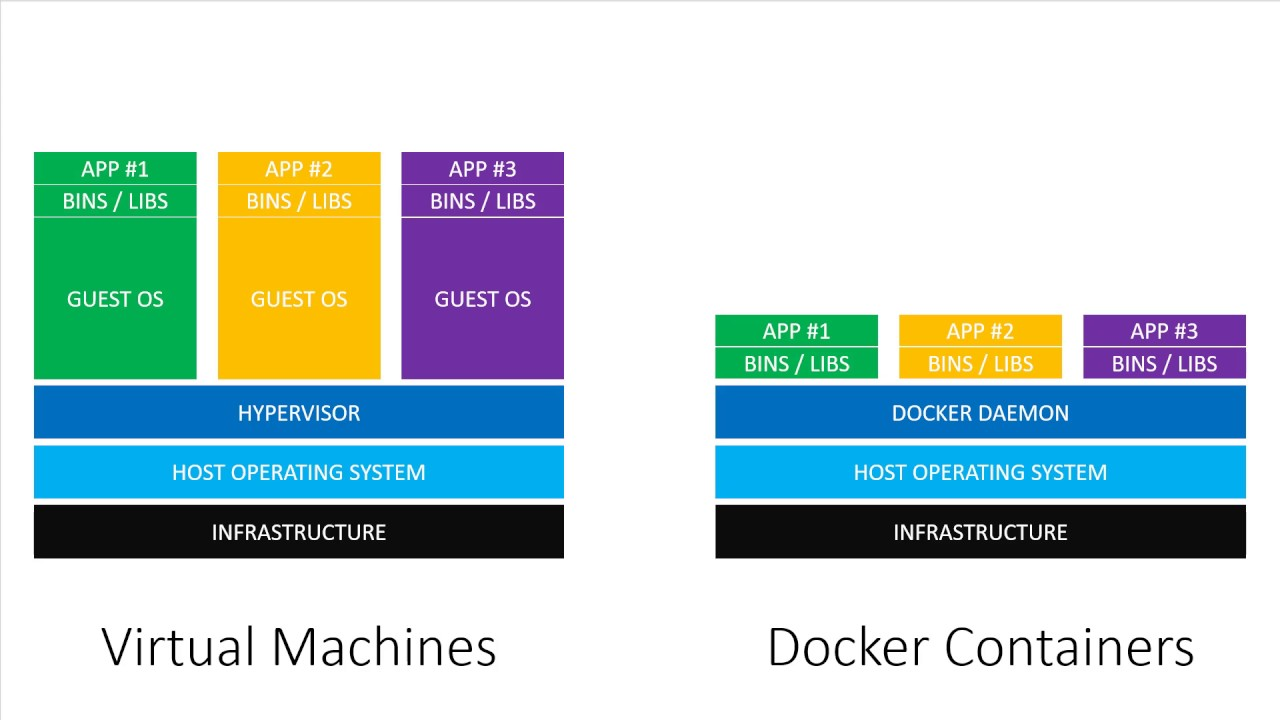
\includegraphics[width=10cm]{img/dockerVSVM.jpg}
\end{frame}

\begin{frame}{Architecture}
    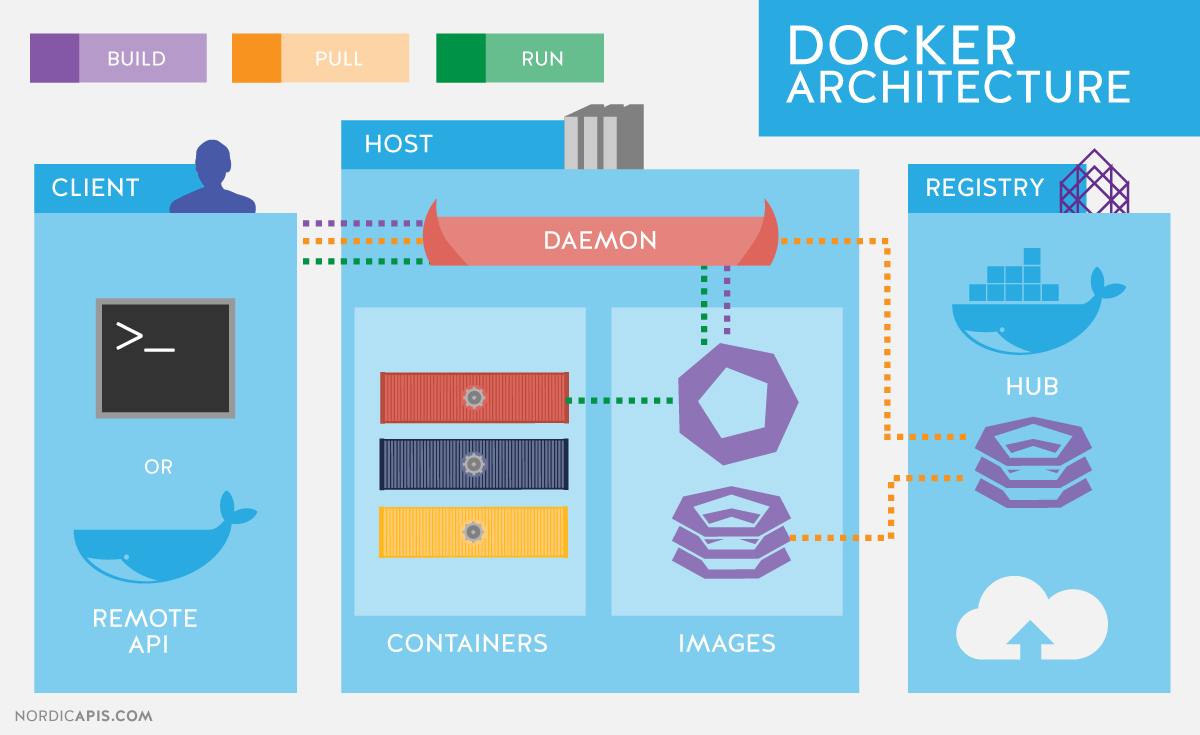
\includegraphics[width=10cm]{img/architecture.png}
\end{frame}

\begin{frame}{Organisation courante}
    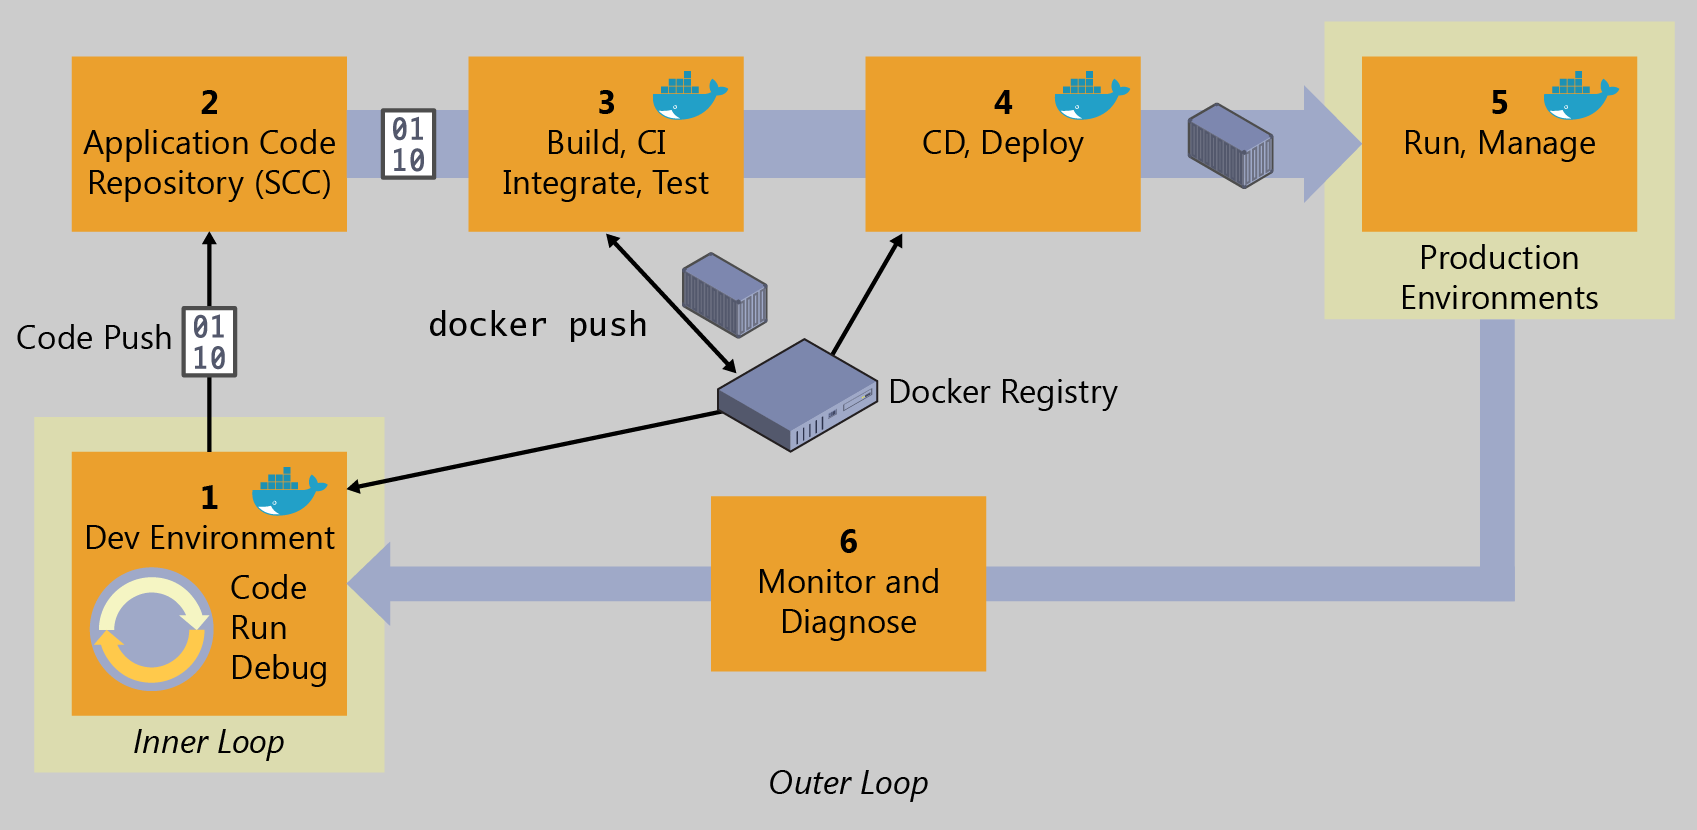
\includegraphics[width=10cm]{img/docker_process.png}
\end{frame}
\end{section}


\begin{section}{DockerHub}
    \begin{frame}{DockerHub}
    \begin{itemize}
        \item Registre d'images publiques docker
        \item \href{https://hub.docker.com}{https://hub.docker.com}
        \item Cible par défaut de docker pull
        \item Permet également de partager des images
    \end{itemize}
\end{frame}
\end{section}


\begin{section}{Mise en place et utilisation}
    \begin{frame}[fragile]{Installation }
    \begin{block}{Pré-requis}
        \begin{itemize}
            \item Virtualisation activée dans le Bios,
            \item minimum 4GB de RAM,
            \item CPU avec capacité SLAT
            \item Windows 10 64bits Pro, Enterprise ou Education / La majeure partie des distributions Linux 64 bits / macOS Sierra 10.12 et plus
        \end{itemize}
    \end{block}
\end{frame}

\begin{frame}{Commandes utiles}
    \begin{itemize}
        \item docker info
        \item docker ps
        \item docker commit
        \item docker build
        \item docker run 
        \item docker image ls
        \item docker container ls --all
    \end{itemize}
\end{frame}
\end{section}

\begin{section}{Orchestration}
    \begin{frame}{Orchestration}
    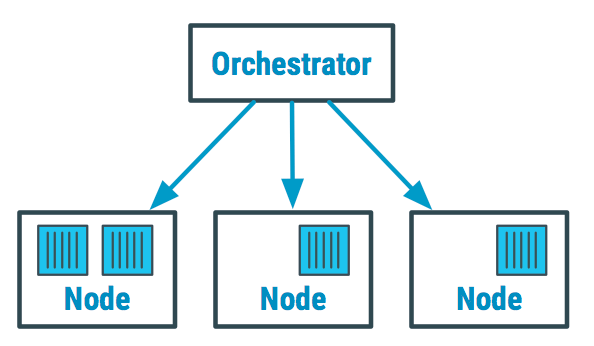
\includegraphics{img/orchestrator.png}
\end{frame}

\begin{frame}[noframenumbering]
    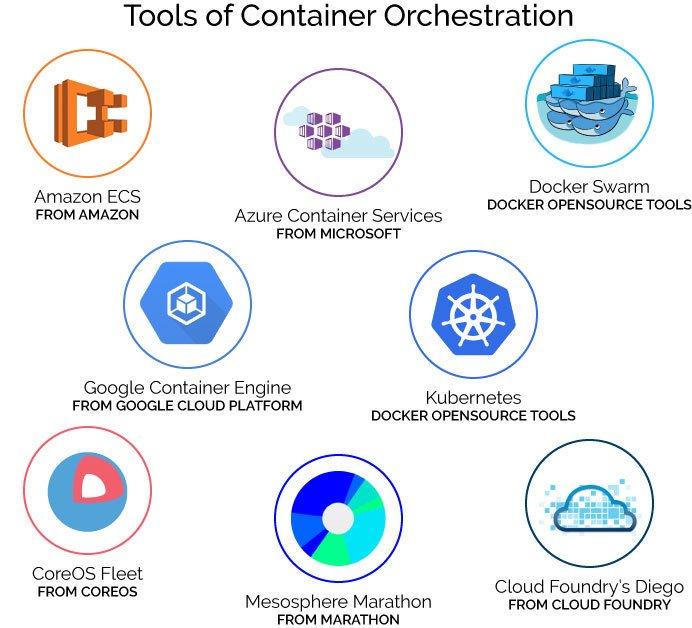
\includegraphics[width=9cm]{img/orchs.jpg}
\end{frame}


\end{section}

\begin{section}{Fichiers exemples}
    \begin{frame}[fragile]{Exemple simple}
    \begin{block}{app.py}
        \begin{verbatim}
From flask import Flask
app = Flask(__name__)
@app.route('/')
def hello_world:
    return 'Hey, we have Flask in a Docker container!'
if __name == '__main__':
    app.run(debug=True, host='0.0.0.0')
\end{verbatim}
    \end{block}
    \begin{block}{requirements.txt}
    Flask==0.10.1
    \end{block}
\end{frame}


\begin{frame}{Exemple simple}
    \begin{block}{DockerFile}
    FROM ubuntu:16.04

MAINTANER Your Name "youremail@domain.tld"

RUN apt-get update -y && \
    apt-get install -y python-pip python-dev

# We copy just the requirements.txt first to leverage Docker cache
COPY ./requirements.txt /app/requirements.txt

WORKDIR /app

RUN pip install -r requirements.txt

COPY . /app

ENTRYPOINT [ "python" ]

CMD [ "app.py" ]
    \end{block}
\end{frame}
\end{section}

\begin{section}{Exemple pratique}
    \begin{frame}{Démonstration}
    \pause
    \begin{block}{}
        Si vous voyez l'ours, tout a bien marché ! 
    \end{block}
        
\includegraphics[width=10cm]{img/bear.jpg}
\end{frame}

\end{section}


\begin{frame}{Merci !}
    Merci de votre attention, si vous avez des questions, n'hésitez pas.
    
    Ces slides sont disponibles sur \href{https://github.com/Freyj/docker-pres}{https://github.com/Freyj/docker-pres} 
    avec les sources qui ont servi à cette présentation.
    
    \begin{columns}
        \begin{column}{0.5\textwidth}
            
\includegraphics[height=3cm]{img/biere.jpg}
        \end{column}
        \begin{column}{0.5\textwidth}
            
\includegraphics[height=3cm]{img/pizza.jpg}
        \end{column}
    \end{columns}
\end{frame}

 \begin{frame}[noframenumbering]{Sources}
 \begin{itemize}
     \item \href{https://en.wikipedia.org/wiki/Docker_(software)}{Page wikipedia sur Docker}
     \item \href{https://www.docker.com/}{Site de Docker, Inc}
     \item \href{https://github.com/docker/docker-ce}{Repo github de docker}
     \item \href{https://www.aquasec.com/wiki/display/containers/}{Documentation sur les containers}
     \item \href{https://www.youtube.com/watch?v=TvnZTi_gaNc}{Origine de l'image slide 5 (vidéo sur la différence VM / Docker)}
 \end{itemize}
 \end{frame}


\end{document}


